\chapter{Solving spin-glass problems using tensor networks}

\section{Introduction to tensor networks}

Benchmarking quantum annealers requires more sophisticated algorithms. \todo{write more intro}
While there exists plethora of general-purpose optimization algorithms, one might hope to achieve better results by exploiting topology of problem's underlying graph and thus locality therein. In this chapter we describe a recent, tensor-network based algorithm for finding low-energy spectrum of Ising spinglasses, designed for problems defined on Chimera-like quasi-two-dimensional graphs. The algorithm exploits sparsity and locality of Chimera graph by representing Boltzmann distribution of spin-glass as a tensor network, whose approximate contraction can be used for computing marginal probability distributions. This procedure can then be combined with well known branch and bound algorithm to iteratively select most promising partial solutions, finally producing an approximation of low-energy spectrum.

\todo[inline,color=SkyBlue]{Mention that the algorithm is physics inspired}
\todo[inline,color=SkyBlue]{Mention the other Chimera-specific algorithm}

\subsection{Branch and bound}
Let us start by considering an Ising spinglass problem defined on a square lattice as depicted in Fig. \ref{fig:lattice-and-border}.  The state space of such system can be viewed as a tree, in which $k$-th level contains all partial configurations $(s_1, \ldots, s_k)$. This representation allows one to explore the state space incrementally in search for low energy states, and possibly prune the less promising branches. In the approach described here, we use marginal probability $p(s_1, s_2, \ldots, s_k)$ as a criterion for deciding which partial configurations are most promising. More precisely, we explore the solution tree in a top-down manner, keeping at most $M$ states at $k$-th level and branching them into $2M$ new partial configurations at level $k+1$ . The new marginal probability distributions can be computed as

\begin{figure}
    \centering
    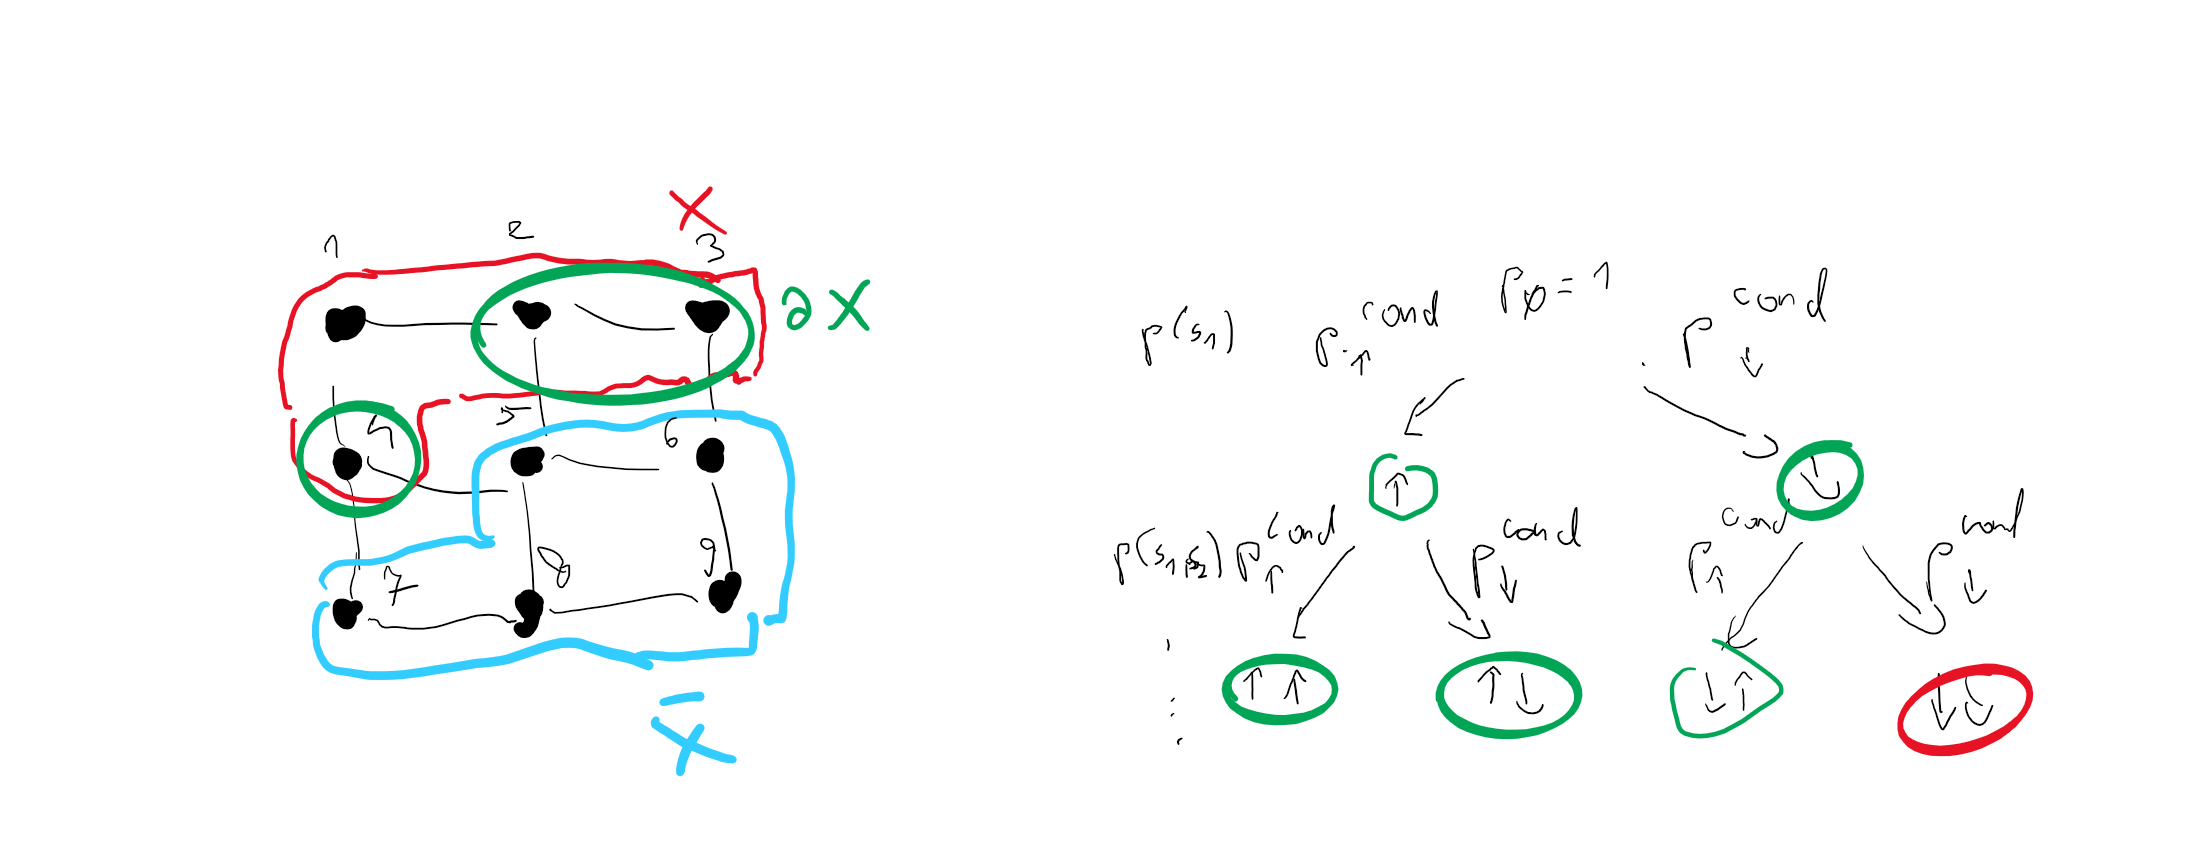
\includegraphics[width=\textwidth]{sketches/lattice.png}
    \caption{\textbf{Left}: Simple system of 9 spins on a square lattice. The border (green) of region $X$ (red) consists of those spins interacting with $\overline{X}$ blue. \textbf{Right}: A fragment of state space tree. States kept at each level are marked with green, and the pruned branches are marked with red.}
    \label{fig:lattice-and-border}
\end{figure}

\begin{equation}
\label{eq:conditional-prob}
    p(s_1, s_2, \ldots, s_k, s_{k+1}) = p(s_1, s_2, \ldots, s_k)p(s_{k+1}|, s_1, \ldots, s_k)
\end{equation}
We can exploit locality of the problem by observing that conditional probability in \eqref{eq:conditional-prob} of configuration in the region $X = (1, 2, \ldots, k)$ depends only on configuration on the border $\partial X$ consisting of those spins, that directly interact with the region $\overline{X} = (k+1, 2, \ldots N)$. To see that, denote by $H_X$ the usual Hamiltonian $H$ restricted to graph induced by vertices in $X$. Further, let $H_{X, \overline{X}} = H - H_X - H_{\overline{X}}$. Notice that $H_{X, \overline{X}}$ contains only quadratic terms $J_{ij} s_i s_j$ such that $i \in X$ and $j \in \overline{X}$. Slightly abusing the notation, one may thus write
\begin{equation}
H(s_1, \ldots, s_N) = H_X(s_1, \ldots, s_k) + H_{\overline{X}}(s_{k+1}, \ldots, s_N) + H_{X, \overline{X}}(s_1, \ldots, s_N)
\end{equation}
Using definition of conditional probability applied to Boltzmann distribution, one thus gets
\begin{align}
    p(s_{k+1}|s_1, \ldots, s_k) &= \frac{\sum\limits_{(z_{k+2}, \ldots, z_N)}e^{-\beta H(s_1, \ldots, s_{k+1}, z_{k+2},\ldots,z_N)}}{\sum\limits_{(z_{k+1}, \ldots, z_N)}e^{-\beta H(s_1, \ldots, s_k, z_{k+1},\ldots,z_N)}} \\
    &= \frac{\sum\limits_{(z_{k+2}, \ldots, z_N)}e^{-\beta (H_X(s_1, \ldots, s_k) + H_{\overline{X}}(s_{k+1}, z_{k+2},\ldots,z_N) + H_{X, \overline{X}}(s_1, \ldots, z_N))}}{\sum\limits_{(z_{k+1}, \ldots, z_N)}e^{-\beta (H_X(s_1, \ldots, s_k) + H_{\overline{X}}(z_{k+1}, \ldots,z_N) + H_{X, \overline{X}}(s_1, \ldots, z_N))}} \\
    & = \frac{e^{-\beta H_X(s_1, \ldots, s_k)}\sum\limits_{(z_{k+2}, \ldots, z_N)} e^{-\beta(H_{\overline{X}}(s_{k+1}, z_{k+2},\ldots,z_N) + H_{X, \overline{X}}(s_1, \ldots, z_N))}}{e^{-\beta H_X(s_1, \ldots, s_k)}\sum\limits_{(z_{k+1}, \ldots, z_N)}e^{ -\beta(H_{\overline{X}}(z_{k+1}, \ldots,z_N) + H_{X, \overline{X}}(s_1, \ldots, z_N))}} \\
    & = \frac{\sum\limits_{(z_{k+2}, \ldots, z_N)} e^{-\beta(H_{\overline{X}}(s_{k+1}, z_{k+2},\ldots,z_N) + H_{X, \overline{X}}(s_1, \ldots, z_N))}}{\sum\limits_{(z_{k+1}, \ldots, z_N)}e^{ -\beta(H_{\overline{X}}(z_{k+1}, \ldots,z_N) + H_{X, \overline{X}}(s_1, \ldots, z_N))}}
\end{align}
Notice that both in numerator and denominator spins with indices from $X$ appear nontrivially only in $H_{X, \overline{X}}$ , i.e. the whole expression depends only on those spins in $X$ that directly interact with spins in $\overline{X}$, which was to be demonstrated.


Before discussing how probabilities in \eqref{eq:conditional-prob} can be computed, let us first extend the above approach to the more general case of a quasi-two-dimensional graph, i.e. one in which nodes can be grouped into \emph{clusters} forming two-dimensional square lattice (see Fig. \ref{fig:quasi2d} for details). One can easily see, that again we can construct a tree-like structure representing state space, this time considering joint configurations of spins in a single cluster. Therefore, for the most of the time we might "forget" the underlying spinglass structure and consider square lattices in which spin clusters act like a higher-dimensional systems.

A central object considered in our algorithm is probability distribution $\exp[-\beta H(\mathbf{s})]$, which we approximate using a PEPS-equivalent tensor network, whose detail will be described shortly. Contracting such network can give probability distribution of any full configuration, as well as the marginal probabilities.

\begin{equation}
    p(s_1, s_2, \ldots, s_k) \sim \tr[\mathcal{P}_{(s_1, \ldots, s_k)} e^{-\beta H(\mathbf{s})}]
\end{equation}

\section{Grouping spins into clusters}
The outlined approach can be easily extended to the case of the problem defined on a graph in which nodes can be grouped into \emph{clusters} forming two-dimensional lattice. See Fig. \ref{fig:quasi2d} for a detailed description. In this more general case, $s_i$ in \eqref{eq:conditional-prob} denote join probability of configuration in $i$-th cluster, and each configuration is branched into $2^lM$ new ones, where $l$ is the number of spins in respective cluster.

\section{PEPS network construction}
We begin construction of PEPS network for quasi-two-dimensional graph by considering two spins at sites $i$ and $j$ connected by an edge $J_{ij}$. This edge can be decomposed as

\begin{equation}
    e^{-\beta J_{ij}s_i s_j} = \sum_{\gamma = \pm 1} B^{s_{i\phantom{j}}}_\gamma C^{s_j}_\gamma
\end{equation}
where 
\begin{equation}
\label{eq:decomposition}
    B^{S_i}_\gamma = \delta_{\gamma s_i} \quad C^{s_j}_\gamma = e^{-\beta \gamma J_{ij} s_j}
\end{equation}
Note that decomposition \eqref{eq:decomposition}, although not unique, has the advantage of comprising only non-negative coefficients, which positively affects numerical stability.
Next, with each cluster we associate a PEPS tensor
\begin{equation}
\label{eq:peps}
A^{\mathbf{s_c}}_{\mathbf{lrud}} = e^{-\beta H(\mathbf{s_c})} B^{\mathbf{s_c}^l}_\mathbf{l}C^{\mathbf{s_c}^r}_\mathbf{r}B^{\mathbf{s_c}^u}_\mathbf{u}C^{\mathbf{s_c}^d}_\mathbf{d}
\end{equation}
Here, $\mathbf{s_c}$ collects all spins in a given cluster, and $\mathbf{s_c}^l$, $\mathbf{s_c}^r$, $\mathbf{s_c}^u$, $\mathbf{s_c}^d$ collect spins interacting with it from the left, right, up and down respectively. Each such tensor has five legs: physical $\mathbf{s_c}$ of dimension $2^m$, where $m$ denotes number of spins in the cluster, and the virtual ones $l, r, u, d$ with dimensions depending on the number of inter-cluster edges. Note that $H$ in \eqref{eq:peps} is restricted to the graph induced by spins belonging to the considered cluster.
\todo[inline,color=green]{Should we mention here, that $H(\mathbf{s_c})$ can be replaced by some approximation scheme?}

% Old stuff below!
\todo[color=red,inline]{The old stuff is below, don't read this}
\begin{figure}
    \centering
    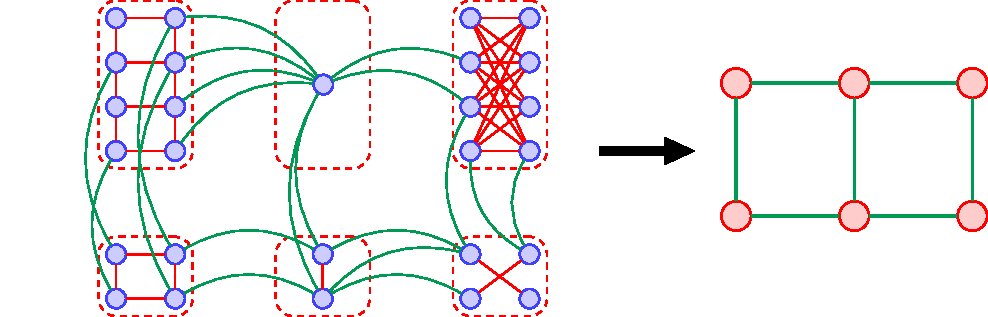
\includegraphics[width=\textwidth]{figures/clustering.pdf}
    \caption{Example quasi-two-dimensional graph that can be used with tensor networks based algorithm presented here. By grouping several spins (variables) together, we converted original graph into two-dimensional lattice. In this view, the green lines represent \emph{intra}cluster edges, whereas blue lines represent \emph{inter}cluster edges.}
    \label{fig:quasi2d}
\end{figure}
We start off by representing the probability distribution $\exp[-\beta H(\mathbf{s})]$ using a PEPS-equivalent tensor network.
Contracting the network can give probability of any full configuration, as well as marginal probabilities

\begin{equation}
    p(s_1, s_2, \ldots, s_k) \sim \tr[\mathcal{P}_{(s_1, \ldots, s_k)} e^{-\beta H(\mathbf{s})}]
\end{equation}
Here, $\mathcal{P}_{(s_1, \ldots, s_k)}$ is a projector on the subspace with a given configuration $(s_1, \ldots, s_k)$.
\todo[inline,color=SkyBlue]{Write marginal probability using conditional probability, show that this depends only on the boundary and not the whole searched configuration}
To this end, with each cluster we associate a tensor
\begin{equation}
A^{\mathbf{s_c}}_{\mathbf{lrud}} = e^{-\beta H(\mathbf{s_c})} B^{\mathbf{s_c}^l}_\mathbf{l}C^{\mathbf{s_c}^r}_\mathbf{r}B^{\mathbf{s_c}^u}_\mathbf{u}C^{\mathbf{s_c}^d}_\mathbf{d}
\end{equation}
Here, $\mathbf{s_c}$ collects all spins in a given cluster, and $\mathbf{s_c}^l$, $\mathbf{s_c}^r$, $\mathbf{s_c}^u$, $\mathbf{s_c}^d$ collect spins interacting with it from the left, right, up and down respectively.

\todo[inline,color=SkyBlue]{Fill in tensor network construcion}

\subsection{Branch and bound}
The state space can be viewed as a tree. In the simplest case, $k$-th level of such tree contains all partial configurations $(s_1, \ldots, s_k)$. The basic idea of extracting low energy spectrum from such a tree is to use branch and bound algorithm. In such an approach, at each step we keep at most $M$ states from the $k$-th level of the tree. Those candidate states are then branched into $2M$ states from $k+1$ level. Instead of considering a single spins, at each tree level one can consider joint configurations of spins in $k-th$ cluster,
which leads to a shorter but wider tree \todo[color=magenta]{This is true, although maybe not necessary to mention here}
\todo[inline,color=SkyBlue]{Mention that we shift from ising to factor graph}
\subsection{Approximate network contraction}
Cost of exact contraction of the proposed network is prohibitively large, therefore, it has to be contracted approximately
After visiting every level of a tree, one is left with an approximation of $M$ lowest energy states. in principle, the algorithm could be used for certifying the solution.